\section{Introduction}\label{sec:intro}\label{sec:notation}

\noindent\begin{minipage}{\linewidth}
\begin{quote}\small\itshape
An elephant and an ant are playing hide and seek. The elephant counts while
the ant hides among many identical anthills, then opens its eyes and knows
at once which one the ant is in. The ant's shoes are outside the door.
\end{quote}
\hfill\textup{(Anonymous)}
\medskip
\end{minipage}

The elephant walk~\cite{schutz2004} has steps $X_i\in\{+1,-1\}$.
Given $X_1,\dots,X_t$, it picks $i$ uniformly from $\{1,\dots,t\}$.
Then $X_{t+1}=X_i$ with probability $1-\varepsilon$, and
$X_{t+1}=-X_i$ otherwise. These choices are independent of each other
and of $X_1$. Put
\[
 A_N=\#\{i\le N:X_i=+1\},\qquad S_N=2A_N-N,\qquad
 P_N(k)=\Prob(A_N=k).
\]
The memory is $a=1-2\varepsilon$ and the initial bias is
$q=\Prob(X_1=1)$. In the original description the copying probability
is $p=(1+a)/2$. After $t$ steps with count $k$, the next step is $+1$
with probability $r_t(k)=\varepsilon+ak/t$. We call $q=1/2$ a fair
start, and $\Prob_+$, $\E_+$ condition on $X_1=1$.

When $a\in(1/2,1)$ the ratio $S_N/N^a$ converges almost surely
\cite{baurbert2016,bercu2018}. Let $h_a$ be the density of the limit
given $X_1=1$. With initial bias $q$ the limit density is
\[
 g_{a,q}(u)=q h_a(u)+(1-q)h_a(-u),\qquad g_a=g_{a,1/2}.
\]
Gu\'erin, Laulin, Raschel, and Simon prove that $h_a$ has one
peak~\cite[Theorem~1.1]{glrs2025}. In~\cite[Remark~2.1(b)]{glrs2025},
they conjecture that $g_{a,q}$ has 2 peaks exactly for $q$ in an open
interval centered at $1/2$, and they describe this problem as
challenging. Our Theorem~\ref{thm:main-limit} answers it with a yes.
Furthermore, our Theorem~\ref{thm:main-analytic} states that the
interval is empty for $a\le a_*$ and nonempty for $a>a_*$, where
$a_*\approx0.6688$.

\subsection{The bias interval and its threshold}\label{sec:results}

\begin{theorem}[the bias interval]\label{thm:main-limit}
For every $a\in(1/2,1)$ there is $b_a\in(0,1/2]$ such that
$g_{a,q}$ has exactly two local maxima if and only if
$b_a<q<1-b_a$. Outside this open interval, including its endpoints,
the density is unimodal with a unique local maximum.
\end{theorem}

In particular $g_{a,q}$ is unimodal for $q\le b_a$ and for
$q\ge1-b_a$. Theorem~\ref{thm:main-analytic} gives the set of $a$ with
$b_a<1/2$.

\begin{theorem}[the analytic threshold]\label{thm:main-analytic}
There is exactly one $a_*\in(2/3,69/100)$ with $g_{a_*}''(0)=0$.
The central curvature is negative below $a_*$ and positive above
it, and $\partial_a g_a''(0)|_{a=a_*}>0$.
The bias interval is empty exactly when $a\le a_*$.
\end{theorem}

Theorem~\ref{thm:main-limit} is Theorems~\ref{thm:two-modes}
and~\ref{thm:biased-limit-modes} together with $b_a>0$ from
Theorem~\ref{thm:bias-continuity}. Theorem~\ref{thm:main-analytic} is
Theorem~\ref{thm:threshold}. These proofs use no computer. The bias
boundary is regular. By Theorem~\ref{thm:bias-continuity}, the function
$a\mapsto b_a$ is continuous on $(1/2,1)$, continuously differentiable
on $(a_*,1)$, and strictly decreasing immediately above $a_*$. By
Corollary~\ref{cor:bias-boundary-rate}, $b_a\to0$ as $a\uparrow1$, and
by Proposition~\ref{prop:quadratic-rate},
$b_a\le82(1-a)^2$ for $a$ close to one. We do not know if $b_a$ is
decreasing on all of $(a_*,1)$ (Section~\ref{sec:open}).

At $a_*$ the fair density has a quartic top
(Lemma~\ref{lem:analytic-quartic}), and the next theorem describes how
the two modes and the bias interval open from it.

\begin{theorem}[the critical exponents]\label{thm:main-critical}
There are positive constants $K_*,Q_*$ such that the positive mode
$\kappa_a$ of $g_a$ and the bias boundary satisfy
\[
 \kappa_a\sim K_*\sqrt{a-a_*},\qquad
 \tfrac12-b_a\sim Q_*(a-a_*)^{3/2}\quad(a\downarrow a_*).
\]
\end{theorem}

The two asymptotics are Propositions~\ref{prop:critical-shape}
and~\ref{prop:bias-cusp}. Theorem~\ref{thm:two-modes} also counts the
inflection points of $g_a$.

\begin{remark}[numerical values]\label{rem:numerics}
Numerically, $a_*\approx0.66881$, $K_*\approx7.2241$, and
$Q_*\approx9.8670$. These values are not used in any proof.
Section~\ref{sec:verify} describes their interval certificates.
\end{remark}

\begin{figure}[t]
\centering
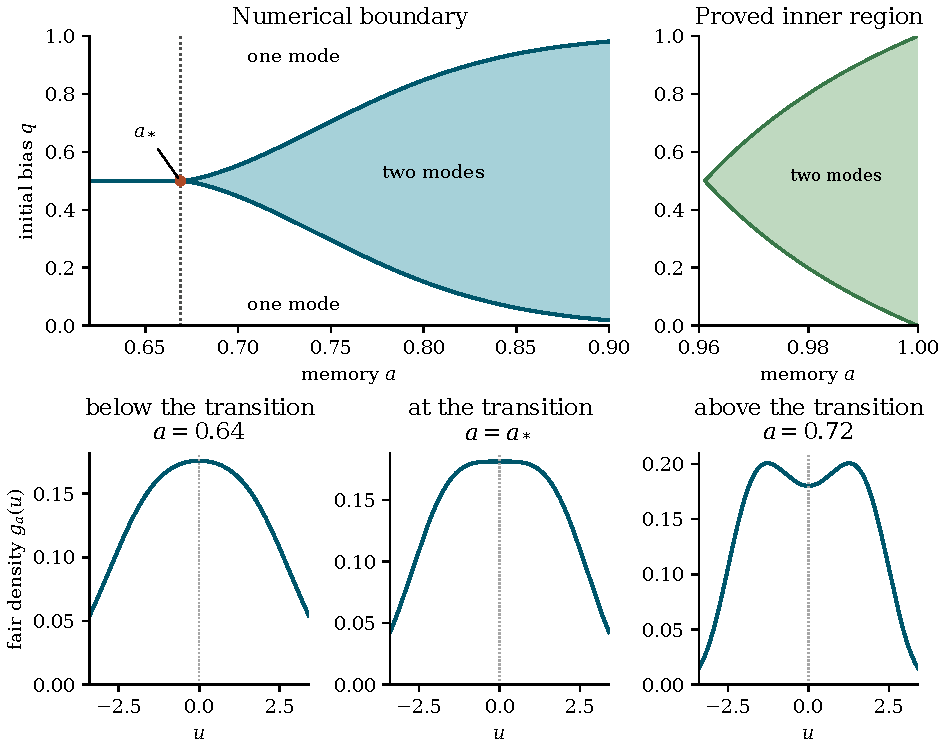
\includegraphics[width=\textwidth]{figures/phase.pdf}
\caption{The bias interval and the fair-start transition. Upper left:
$b_a$ and $1-b_a$ from Theorem~\ref{thm:bias-continuity}, computed
numerically (not certified). Upper right: the region
$4\rho_a/(1-4\rho_a)<q<1-4\rho_a/(1-4\rho_a)$ of
Corollary~\ref{cor:bias-boundary-rate}, which is contained in the
interval. Lower row: $g_a$ for $a=0.64$, $a=a_*$, and $a=0.72$. The top
at $a_*$ is quartic by Lemma~\ref{lem:analytic-quartic}.}
\label{fig:phase}
\end{figure}

\subsection{From finite signs to the limiting shape}\label{sec:architecture}

Gu\'erin, Laulin, Raschel, and Simon prove unimodality by induction on
$N$ for the count law, given $X_1=1$. We do the same induction on every
$q$. By~\eqref{eq:D-rec}, for $2\le k\le t-1$ the value $D_{t+1}(k)$ is
a positive combination of $D_t(k-1)$ and $D_t(k)$. By
Lemma~\ref{lem:interleave}, this step adds no sign change. The new
problem lies at the two ends of a row, because
$D_{t+1}(1)=D_{t+1}(t)=s_{t+1}$ is new, and any value added to the end
can induce a sign change. Hence, we fix the final length $N$ and write
the boundary values $s_N,\dots,s_{t+1}$ entering before time $N$ on
both sides of row $t$. Lemma~\ref{lem:level-one} bounds the signs of
$(s_3,\dots,s_N)$, and then the induction runs over the whole longer
row (Theorem~\ref{thm:five-blocks}). For an arbitrary bias we do the
same with first differences (Figure~\ref{fig:augmented-rows}). By
Proposition~\ref{prop:all-bias-modes}, the first differences within
this longer row swap signs at most 3 times. By
Lemma~\ref{lem:derivative-limits}, all these bounds pass to $g_a$,
$g_a'$, and $g_a''$.

Let $q\ge1/2$. Proposition~\ref{prop:dominant-half} eliminates the
possibility of a $-$ and then a $+$ on the right half. So on
$[0,\infty)$ the density $g_{a,q}$ has no strict valley, and
$g_{a,q}(-x)\le g_{a,q}(x)$. Hence $g_{a,q}$ has two peaks if and only
if $g_{a,q}(x)>g_{a,q}(y)$ for some $x<y\le0$. For fixed $x,y$ this
difference is affine in $q$ and is $\le0$ at $q=1$. If it is positive
at some $q$, it is positive on $[1/2,q]$. Taking the union over $x,y$
and reflecting gives an interval $(b_a,1-b_a)$
(Theorem~\ref{thm:biased-limit-modes}). By
Lemma~\ref{lem:positive-conditional-mode}, $h_a'(0)>0$ for every
$a\in(1/2,1)$, and we can conclude $b_a>0$.

For $a_*$, let $E$ be an independent exponential variable. The
moments of $E^a\mathcal L_a$, where $\mathcal L_a$ is the limit of
$S_N/N^a$ given $X_1=1$, give the transform
of~\cite[Proposition~3.2]{glrs2025}. Two integrations by parts in its Mellin transform give
$g_a''(0)$ as a positive multiple of $\mathcal R(a)-1$, where
$\mathcal R(a)$ is a weighted mean against a positive weight
(Lemma~\ref{lem:curvature-weight}). Rational bounds give the sign of
$g_a''(0)$ for $a\notin[2/3,69/100]$. On $[2/3,69/100]$ the score of
the weight is increasing in the integration variable, and a covariance
identity gives $\mathcal R'(a)>0$
(Appendix~\ref{app:analytic-threshold}). Hence $g_a''(0)$ changes sign
exactly once as $a$ increases (Theorem~\ref{thm:threshold}). The
boundary histories and this positive-weight integral are the new parts
of the argument.

\subsection{Prior work}\label{sec:prior}

The counting chain predates the elephant walk. The Drezner--Farnum
model~\cite{dreznerfarnum1993}, in the formulation of
James, James, and Qi~\cite[p.~2339]{jamesjamesqi2008}, has
next-success probability $(1-\theta)p+\theta k/t$.
With $p=1/2$ and $\theta=a$ this is $r_t(k)$. Their family contains
bimodal laws. Heyde~\cite{heyde2004} gives the limit regimes at fixed
parameters, and James, James, and Qi allow $\theta$ to depend on $t$.
Baur and Bertoin~\cite{baurbert2016} prove functional limit theorems
through P\'olya-type urns. Its memory structure is a random recursive
tree~\cite{kursten2016}, and the split of this tree into two subtrees
is used in Appendix~\ref{app:modes}. Zeros and recurrence of the walk
are studied in~\cite{bertoin2022,qin2025}. See
also~\cite{coletti2017,bercu2018,kubotatakei2019}.

We use the density and moments from~\cite[Theorems~1.3 and~1.4]{glr2026}
and conditional unimodality from~\cite[Theorem~1.1]{glrs2025}. Kiss
and Vet\H{o}~\cite{kissveto2022} compute the first moments for
general steps. Transition probabilities, Gaussian rates, and moment
recurrences are in the preprints
\cite{peresqin2026,muraharatokumitsu2026,vishwakarma2026}.
Trinas and Valle~\cite{tv2026} prove a superdiffusive local limit
theorem, and show the conditional law is not log-concave. Their
difference recurrence also gives Lemma~\ref{lem:derivative-limits}.
Since their paper is a preprint, we include the proof. Trinas~\cite{trinas2026}
uses their local limit theorem for the last-return law, in which the
value $g_{a,q}(0)$ appears.

Da Silva, Cressoni, Sch\"utz, Viswanathan, and
Trimper~\cite{dasilva2013} showed that the superdiffusive propagator is
not Gaussian. In a growing-network model, Mohandas et
al.~\cite[Section~V and Figure~5]{mohandas2025} found the
fair-start transition numerically. They extrapolated finite-$N$
central curvatures and got copying probability about $0.836$. In
their parameter, $a_*$ corresponds to $(1+a_*)/2\approx0.8344$.

The weights giving two peaks are known for normal
mixtures~\cite{eisenberger1964,robertsonfryer1969}, but $h_a$ is not
Gaussian, and the interior step of our induction is classical variation
diminution~\cite{karlin1968,karlin1964}.
